\chapter{Robotic Manipulator Kinematic}
In robotic manipulator, we are interest in position of robot's end effector. It is a mapping from joint space to task space.

\section{Kinematic Chain}
A robot manipulator with $n$ joints will have $n + 1$ links, since each joint connects two links. We number the joints from 1 to $n$, and we number the links from 0 to $n$, starting from the base. By this convention, joint $i$ connects link $i - 1$ to link $i$. We will consider the location of joint $i$ to be fixed with respect to link $i - 1$. When joint $i$ is actuated, link $i$ moves. Therefore, link 0 (the first link or base) is fixed, and does not move when the joints are actuated.
\begin{figure}[ht]
	\centering
	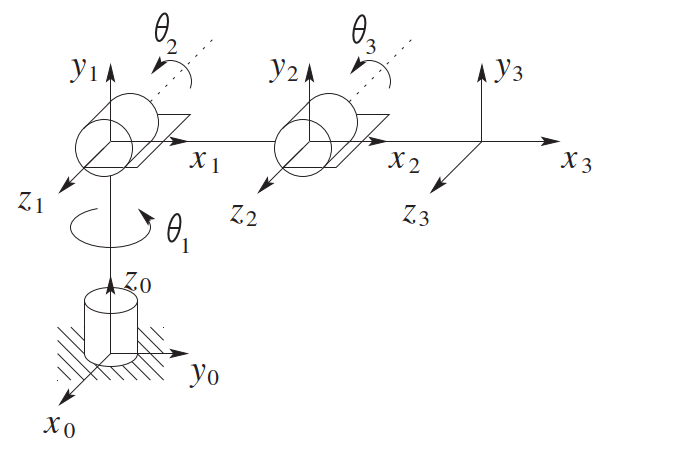
\includegraphics[width=0.5\linewidth]{src/arm/armfig1.png}
\end{figure}
\paragraph{Joint Variable} We assume that each joint has 1 DOF. Thus we have joint variable parameter as:
\[
q_i =
\begin{Bmatrix}
	\theta_i \text{ for revolute joint}\\
	d_i \text{ for prismatic joint}
\end{Bmatrix}
\]
Homogeneous transformation matrix is the function of joint variable:
\begin{equation}
	H_i = H_i(q_i)
\end{equation}
Than we have our transformation matrix:
\begin{equation}
	T_j^i = 
	\begin{Bmatrix}
		H_{i+1} H_{i+2}...H_{j-1} Hj  \\
		I \\
		(T_j^i)^{-1} 
	\end{Bmatrix}
	\begin{matrix}
		\text{ if } i<j\\
		\text{ if } i=j\\
		\text{ if } i>j
	\end{matrix}
\end{equation}
\paragraph{Homogeneous Transformation Matrix}
\begin{equation}
	H =
	\begin{bmatrix}
		R_n^0 && O_n^0 \\
		0 && 1
	\end{bmatrix}
\end{equation}
Position and orientation of end effector in inertial frame is given by:
\begin{equation}
	T_n^0 = H_1(q_1)...H_n(q_n) =
	\begin{bmatrix}
		R_1^0 && O_1^0 \\
		0 && 1
	\end{bmatrix}...
	\begin{bmatrix}
		R_{n-1}^n && O_{n-1}^n \\
		0 && 1
	\end{bmatrix}
\end{equation}
Each component of transformation matrix are:
\begin{equation}
	\begin{split}
		R_j^i &= R_{i+1}^i ... R_{j}^{j-1} \\
		O_j^i &= O_{j-1}^i + R_{j-1}^i O_j^{j-1}
	\end{split}
\end{equation}

\section{Danavit-Hartenberg Convention}
In the convention, the transformation matrix $H$ can be represent as a product 4 basic transformations. An arbitrary homogeneous transformation matrix can be characterized by six numbers, three numbers to specify the fourth column of the matrix and three Euler angles to specify the upper left 3 × 3 rotation matrix. In the DH representation, there are only four parameters. How is this possible? Yes, by choice of the origin and the coordinate axes, it is possible to cut down the number of parameters needed from six to four.
\begin{equation}
	\begin{split}
		H_i &= Rot_{z,\theta_i}Trans_{z,d_i}Trans_{x,a_i}Rot_{x,\alpha_i}\\
		&=\begin{bmatrix}
			c\theta_i & -s\theta_i & 0 & 0\\
			s\theta_i &  c\theta_i & 0 & 0\\
			0  & 0 &  1 & 0\\
			0  & 0 &  0 & 1
		\end{bmatrix}
		\begin{bmatrix}
			1 & 0 & 0 & 0\\
			0 & 1 & 0 & 0\\
			0 & 0 & 1 & d_i\\
			0 & 0 & 0 & 1
		\end{bmatrix}
		\begin{bmatrix}
			1 & 0 & 0 & a_i\\
			0 & 1 & 0 & 0\\
			0 & 0 & 1 & 0\\
			0 & 0 & 0 & 1
		\end{bmatrix}
		\begin{bmatrix}
			1 & 0 & 0 & 0\\
			0 & c\alpha_i & -s\alpha_i & 0\\
			0 & s\alpha_i & c\alpha_i & 0\\
			0 & 0 & 0 & 1
		\end{bmatrix}\\
	 &=\begin{bmatrix}
	 	c\theta_i & -s\theta_ic\alpha_i & s\theta_i s\alpha_i & a_ic\theta_i\\
	 	s\theta_i & c\theta_i c\alpha_i & -c\theta_i s\alpha_i & a_i s\theta_i\\
	 	0 & s\alpha_i & c\alpha_i & d_i\\
	 	0 & 0 & 0 & 1
	 \end{bmatrix}
	\end{split}
\end{equation}
Where:
\begin{itemize}
	\item {\makebox[1cm]{$a_i$\hfill} link length}
	\item {\makebox[1cm]{$\alpha_i$\hfill} link twist}
	\item {\makebox[1cm]{$d_i$\hfill} link offset}
	\item {\makebox[1cm]{$\theta_i$\hfill} joint angle}
\end{itemize}





\section{Two Revolute Joint Plannar}
\subsection{Forward Kinematic with Geometrical Approach}

Figure here\hfil

The coordinate of the end effector are:
\begin{equation}
	\begin{split}
		x &= a_1 \cos \theta_1 + a_2 \cos(\theta_1+\theta_2)\\
		y &= a_1 \sin \theta_1 + a_2 \sin(\theta_1+\theta_2)
	\end{split}
\end{equation}
\paragraph{Rotation} We can get a rotation matrix from frame 2 to frame 0 by:
\begin{equation}
	\begin{bmatrix}
		x_2.x_0 & y_2.x_0 \\
		x_2.y_0 & y_2.y_0 
	\end{bmatrix}=
	\begin{bmatrix}
		\cos (\theta_1+\theta_2) & -\sin (\theta_1+\theta_2) \\
		\sin (\theta_1+\theta_2) & \cos (\theta_1+\theta_2)
	\end{bmatrix}
\end{equation}


\subsection{Inverse Kinematic with Geometrical Approach}
From some trigonometry stuff, we can get inverse kinematic. But in robot with more joint, it is not wise to use this approach since the robot can have more to infinite solution (redundant robot). For our Two Revolute Joint Plannar, we have:
\begin{equation}
	\begin{split}
		\theta_2 &= \tan^{-1} (\frac{\pm \sqrt{1-D^2}}{D}) \\
		\theta_1 &= \tan^{-1}(y/x) - \tan^{-1} (\frac{a_2 \sin \theta_2}{a_1 + a_2 \cos \theta_2})
	\end{split}
\end{equation}

\subsection{Velocity Kinematic}
Relation of tool velocity and joint velocity with respect to time. From:
\begin{equation}\label{key}
	\dot{x}(\theta) = \sum_{i=1}^{n} \frac{\partial x}{\partial \theta_i} \frac{\partial \theta_i}{\partial t} = \sum_{i=1}^{n} \frac{\partial x}{\partial \theta_i} \dot{\theta_i}(t) = \frac{\partial x}{\partial \theta_1}\dot{\theta_1}(t) + \frac{\partial x}{\partial \theta_2}\dot{\theta_2}(t) + ... + \frac{\partial x}{\partial \theta_n}\dot{\theta_n}(t)
\end{equation}
We get:
\begin{equation}
	\begin{split}
		\frac{\partial x}{\partial \theta_1} &= -a_1 \sin \theta_1 - a_2 \sin(\theta_1+\theta_2) \\
		\frac{\partial x}{\partial \theta_2} &= 0 - a_2 \sin(\theta_1+\theta_2) \\
		\frac{\partial y}{\partial \theta_1} &= a_1 \cos \theta_1 + a_2 \cos(\theta_1+\theta_2) \\
		\frac{\partial y}{\partial \theta_2} &= 0 + a_2 \cos(\theta_1+\theta_2) \\
	\end{split}
\end{equation}
We get:
\begin{equation}
	\begin{bmatrix}
		\dot{x} \\
		\dot{y} 
	\end{bmatrix}=
	\begin{bmatrix}
		-a_1 \sin \theta_1 - a_2 \sin(\theta_1+\theta_2) & - a_2 \sin(\theta_1+\theta_2) \\
		a_1 \cos \theta_1 + a_2 \cos(\theta_1+\theta_2) & a_2 \cos(\theta_1+\theta_2)
	\end{bmatrix}
	\begin{bmatrix}
		\dot{\theta_1} \\
		\dot{\theta_2} 
	\end{bmatrix}
\end{equation}
Than we may write the about equation as:
\begin{equation}
	\dot{x} = J\dot{\theta}
\end{equation}
Because of relationship of linear velocity $\dot{x}$ to joint velocity $\dot{\theta}$ is linear by Jacobian Matrix $J$, it is conceptually simple to find inverse Jacobian.
\paragraph{Inverse Jacobian}
\begin{equation}
	\begin{split}
		\dot{\theta} &= J^{-1}\dot{x}\\
		J^{-1} &= \frac{1}{\det(J)} adj(J)\\
		J^{-1} &= \frac{1}{a_1a_2\sin\theta_2}
		\begin{bmatrix}
			a_2\cos(\theta_1+\theta_2) & a_2\sin(\theta_1+\theta_2) \\
			-a \cos\theta_1-a_2\cos(\theta_1+\theta_2) & -a\sin\theta_1-a_2\sin(\theta_1+\theta_2)
		\end{bmatrix}
	\end{split}
\end{equation}
If we have a look at the term \(\frac{1}{a_1a_2\sin\theta_2}\), we see that if $\theta_2 = 0 \rightarrow \sin\theta_2 = 0 , \pi$. This make $J$ has no inverse which is said to be Singularity Matrix. Take a look at the figure:

Figure Here

The robot cannot move to direction of $-x$ because it is block by arm link. And we always want to avoid this situation when do planning.

\subsection{Forward Kinematic with DH Approach}
Figure here
\paragraph{DH Table}

\begin{tabular}{|c|c|c|c|c|}
	\hline
	Link & $a_i$ & $\alpha_i$ & $d_i$ & $\theta_i$ \\
	\hline
	1 & $a_1$ & 0 & 0 & $\theta_1$ \\
	1 & $a_2$ & 0 & 0 & $\theta_2$ \\
	\hline
\end{tabular}

The transformation matrices are:
\[
\begin{split}
	T_1^0 &= H_1 \\
	T_2^0 &= H_1H_2 = 
	\begin{bmatrix}
		c\theta_1\theta_2 & -s\theta_1\theta_2 & 0 & a_1c\theta_1+a_2c\theta_1\theta_2\\
		s\theta_1\theta_2 & c\theta_1\theta_2 & 0 & a_1s\theta_1+a_2s\theta_1\theta_2\\
		0 & 0 & 1 & 0\\
		0 & 0 & 0 & 1
	\end{bmatrix}
\end{split}
\]